
\section{Introduction}
\label{sec:intro}

\noindent {\bf Big Data Brings Multi-tenancy:}
It has become essential for companies to process large amounts of data (popularly called {\em big data} today). Efficient processing of big data requires moving computation to the data, thereby requiring application code to run on the same machines where the data resides. Consequently, the need to process big data leads to multi-tenancy in which multiple applications run on and share the same resources and data \cite{mesos,yarn,ghodsi11,isard09}.

\noindent {\bf Multi-tenancy Breeds Heterogeneity:}
The various tenants in a multi-tenant big data deployment are seldom 
homogeneous in their behavior and performance requirements.
Heterogeneity can arise along multiple dimensions: 

\squishlist

\item Applications may create different types of workloads, from ad-hoc, interactive queries, to workflows that recur at different frequencies, with varying complexities.

\item Applications may create and analyze different data sets varying in their data types, volume, and velocity.

\item Applications may use different high-level platforms (e.g., Hive, Pig), computational engines (e.g., MapReduce, Spark, Tez), workflow scheduling mechanisms (e.g., Oozie), and graph processing systems (e.g., Giraph).

\item Applications may be created by a user base with a diverse set of skills and expectations, such as computer scientists, statisticians, and business analysts.

\item Last, but not least, applications may have conflicting performance requirements, such as low latency, high throughput, large I/O, large amounts of memory, and rapid application development cycles.

\squishend 

\begin{figure*}[t!]
        \centering
        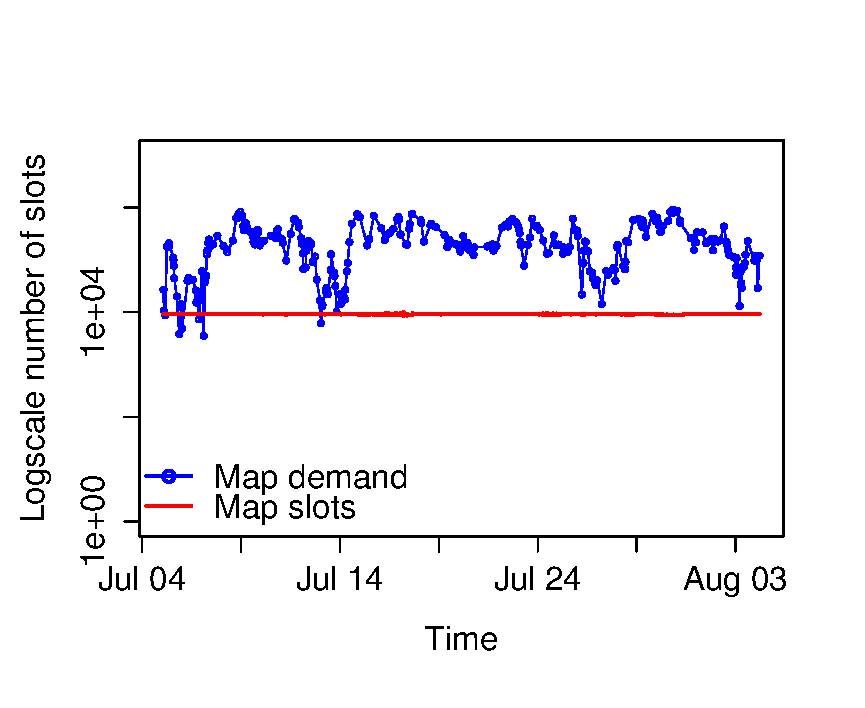
\includegraphics[width=.3\textwidth]{map_demand_and_slots.eps}
        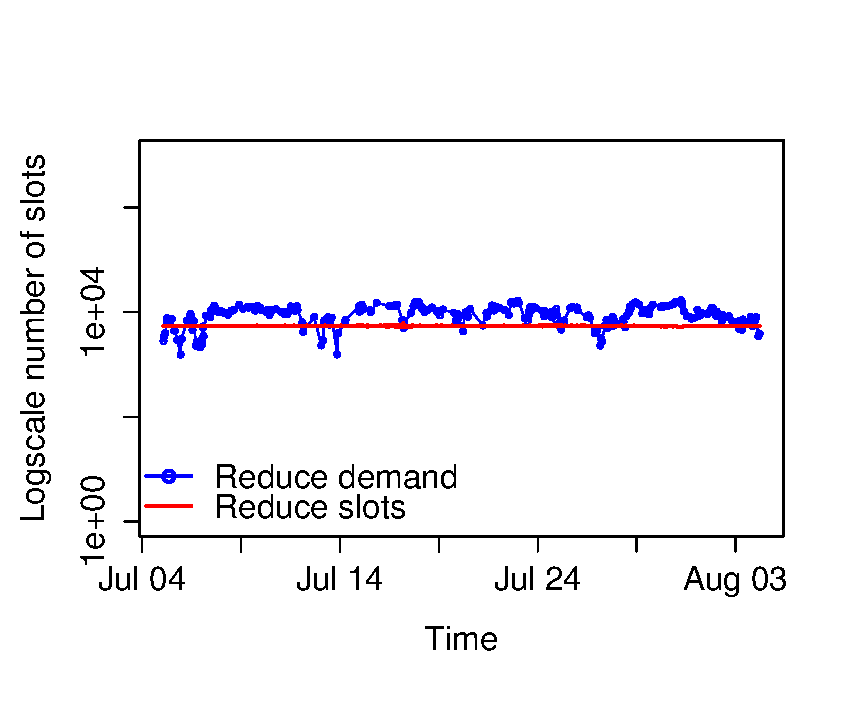
\includegraphics[width=.3\textwidth]{reduce_demand_and_slots.eps}
        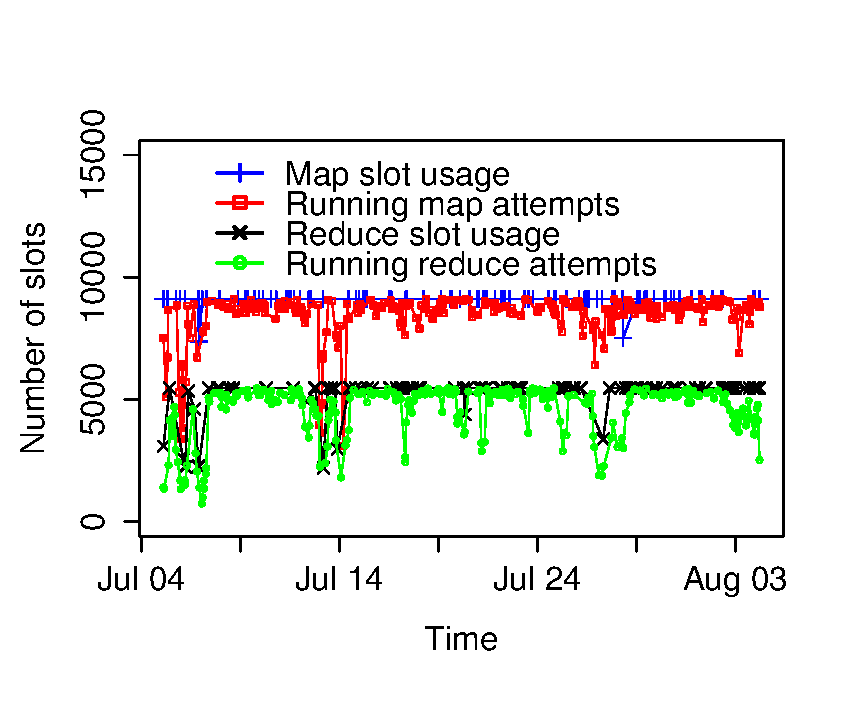
\includegraphics[width=.3\textwidth]{demand_and_running.eps}
        \vspace{-4mm}
        \caption{(a) Map demand (log-scale), (b) Reduce demand (log-scale), and (c) 
 Resource usage on the cluster}
        \vspace{-6mm}
        \label{fig:demand}
\end{figure*}

\noindent {\bf Gatekeepers of Multi-tenancy:}
To meet the conflicting requirements amid different kinds of heterogeneity in a multi-tenant big data system, various mechanisms are used to control how resources are allocated to the applications sharing the cluster. A common technique is to map applications to a set of {\em pools}. Policies are then defined to determine: (a) How are resources distributed across different pools? (b) When is an application admitted to use resources assigned to its pool? (c) How are resources distributed across different applications in the same pool?

These policies can have a huge impact on the performance of a multi-tenant cluster. However, defining policies to achieve good performance is extremely challenging because of the conflicting requirements and the complexities of the system and multi-tenancy. Unfortunately, in practice this responsibility often falls largely on the operations team that manages the cluster, with few effective tools to make data-driven decisions. 

In this paper, we use operational experiences from a large multi-tenant cluster at Rocket Fuel to discuss challenges that operators of these clusters face. Rocket Fuel has a fast-growing Hadoop cluster that currently stores approximately 30 petabytes of data across more than 1000 nodes. Almost all the above types of heterogeneity are seen in this cluster. We break down the challenges in the form of questions that these operators have to answer routinely.  For example:

\squishlist

\item {\em What is the effective utilization of my cluster?} 
We will show in Section \ref{sec:sec2} that the effective utilization of a multi-tenant cluster can be much less than what cluster operators would think based on typical monitoring tools for resource usage.  

\item {\em Should preemption be turned on?} 
The ability for an application X to pre-empt another application Y and start using the resources allocated to Y is one of the configurable policies in multi-tenancy; however, if not used wisely, preemption could lead to significant wasted time and resources.

\item {\em What will be the overall impact of a 10\% increase
in the workload of Pool A?}  
We will show in Section \ref{sec:sec2} that a small increase in the workload of a pool can have a major impact on the performance of applications in another pool in a multi-tenant cluster.

\item {\em What will be the overall impact of changing the data layout
of a table T?}  The application that populates $T$ may belong to a different pool from applications that read from $T$; which in turn could be used to build more tables used by other applications from any pool. These dependencies make the problem of tuning data layouts in a multi-tenant cluster highly challenging.

\squishend

\noindent {\bf Contributions and Roadmap:} 
The above examples come from a large space of questions that human operators have to answer in order to manage multi-tenant clusters effectively. To the best of our knowledge, no single solution exists today that allows operators to ask these questions and get data-driven answers automatically. This paper presents {\em Colossal}, a solution that we have created for this 
problem.

We use real-life examples in Section \ref{sec:sec2} to motivate the challenges that operators of multi-tenant clusters face. Section \ref{sec:sec3} presents Colossal. Section \ref{sec:sec4} discusses related work
and concludes the paper.
